\setcounter{section}{2}
\setcounter{dang}{0}
\section{Phương trình đường thẳng}
\Opensolutionfile{ans}[ans/ans-DT03]
\subsection{Tóm tắt lý thuyết}

\subsubsection{Phương trình tổng quát của đường thẳng}

\textbf{vectơ pháp tuyến của đường thẳng}
	\immini{vectơ $\overrightarrow{n} \ne \overrightarrow{0}$ được gọi là vectơ pháp tuyến  (VTPT) của đường thẳng $\Delta$ nếu giá của nó vuông góc với $\Delta$.
	}{
	\begin{tikzpicture}[scale=1, font=\footnotesize, line join=round, line cap=round, >=stealth]
		\draw (0,0)--(3,0) node[right] {$\Delta$} ;
		\draw[->,line width =1pt] (1,0)--(1,1)  node[above] {$\overrightarrow{n}_{\Delta}$} ;
		\draw (0.8,0)|- (1,.2);
	\end{tikzpicture}
	}
	Nhận xét
	\begin{itemize}
		\item Nếu vectơ $\overrightarrow{n}$  là một VTPT của $\Delta$ thì $k \overrightarrow{n}$ ($k \ne 0 $) cũng là một VTPT của $\Delta$. 
		\item Một đường thẳng hoàn toàn được xác định nếu biết một điểm và một VTPT.
	\end{itemize}

\textbf{Phương trình tổng quát của đường thẳng}
	Cho đường thẳng $\Delta$ đi qua $M(x_0;y_0)$ và có VTPT $\overrightarrow{n}_{\Delta} (a;b)$. Phương trình tổng quát của $\Delta$ là 
	$$\Delta \colon a(x-x_0) +b(y-y_0) = 0 \text{ hay } ax+by+c=0 ~(\text{với } c=-ax_0-by_0).$$

 Một số trường hợp đặc biệt
	\begin{center}
		\renewcommand{\arraystretch}{2}%điều chỉnh khoảng giãn cách giữa các hàng,mặc định là 1	
		\begin{tabular}{|c|c|c|}
			\hline 
			Các hệ số & PTĐT $\Delta$ & Tính chất đường thẳng $\Delta$ \\ 
			\hline 
			$c=0$ & $ax+by =0$ & $\Delta$ đi qua gốc tọa độ $O$ \\ 
			\hline 
			$a=0$ & $by+c=0$ & $\Delta \parallel Ox$ hoặc $\Delta  \equiv Ox$ \\ 
			\hline 
			$b=0$ & $ax+c=0$ &  $\Delta \parallel Oy$ hoặc $\Delta  \equiv Oy$ \\ 
			\hline 
		\end{tabular} 
	\end{center}


\begin{note}
	Đồ thị hàm số bậc nhất $y=ax+b$ chính là đường thẳng $ax-y+b=0$ (không vuông góc với trục $Ox$).
\end{note}

\subsubsection{Phương trình tham số của đường thẳng}
\textbf{vectơ chỉ phương của đường thẳng}
	\immini{
	vectơ $\overrightarrow{u} \ne \overrightarrow{0}$ được gọi là vectơ chỉ phương (VTCP) của đường thẳng $\Delta$ nếu giá của nó song song hoặc trùng với $\Delta$.
	}{
	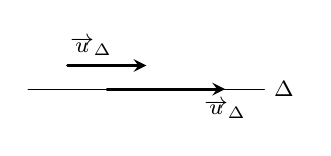
\begin{tikzpicture}[scale=1, font=\footnotesize, line join=round, line cap=round, >=stealth]
		\draw (0,0)--(3,0) node[right] {$\Delta$} ;
		\draw[->,line width =1pt] (1,0)--(2.5,0)  node[below] {$\overrightarrow{u}_{\Delta}$} ;
		\draw[->,line width =1pt] (0.5,0.3)--(1.5,0.3) ; 
		\draw (0.8,0.3)node[above] {$\overrightarrow{u}_{\Delta}$} ;
	\end{tikzpicture}
	}
		Nhận xét 
		\begin{itemize}
			\item Nếu vectơ $\overrightarrow{u}$  là một VTCP của $\Delta$ thì $k \overrightarrow{u}$ ($k \ne 0 $) cũng là một VTCP của $\Delta$. 
			\item Một đường thẳng hoàn toàn được xác định nếu biết một điểm và một VTCP.
			\item Nếu $\overrightarrow{u}$ là một VTCP và $\overrightarrow{n}$ là một VTPT của $\Delta$ thì $\overrightarrow{u} \perp \overrightarrow{n}$.
		\end{itemize}
		
\textbf{PTTS của đường thẳng}
	Cho đường thẳng $\Delta $ đi qua $M(x_0;y_0)$ và có VTCP $\overrightarrow{u}(u_1;u_2)$. PTTS của $\Delta $ là
	$$\Delta \colon \heva{&x= x_0 +  u_1 t\\&y =y_0 +u_2 t} ~(\textrm{với } t \textrm{ là tham số và } t \in \mathbb{R} ).$$
		 Nhận xét 
		\begin{itemize}
			\item[+] $M(x_M;y_M) \in \Delta \Leftrightarrow \exists t \in \mathbb{R} \colon \heva{&x_M= x_0 + t u_1\\&y_M =y_0 +tu_2}$ hay 
			$M(x_0 +tu_1 ; y_0 +tu_2) \in \Delta$. 
			\item[+] Gọi $k$ là hệ số góc của $\Delta$ có VTCP $\overrightarrow{u}(u_1;u_2)$ thì 
			\immini{
				$\bullet$  $k= \tan \alpha$ với $\heva{&\alpha =\widehat{xAt}\\&\alpha \ne 90^\circ.}$ \\
				$\bullet$ $k= \dfrac{u_2}{u_1}$ với $u_1 \ne 0$. 
			}{
				\begin{tikzpicture}[scale =0.6, font=\footnotesize, line join=round, line cap=round, >=stealth]
					\tkzDefPoints{-1/-2/X,3/2/Y,3/0/Z,1/0/A}
					\draw[->] (-1,0)--(3,0) node[right] {$x$} ;
					\draw[->] (0,-1.5)--(0,1.5) node[above] {$y$} ;
					\draw[fill=black] (0,0) circle (1.2pt) node[below left=-2pt] {$O$};
					\draw[fill=black] (1,0) circle (1.2pt) node[above left=-2pt] {$A$};
					\draw (2.5,1.5) node[above] {$t$};
					\tkzMarkAngle[arrows=->,size=0.9](Z,A,Y)
					\tkzLabelAngle[pos=0.6](Z,A,Y){\small $\alpha$}
					\clip (-1,-1.5) rectangle (3,1.5) ;
					\draw (X)--(Y) ;
				\end{tikzpicture} \quad 
				\begin{tikzpicture}[scale =0.6,>=stealth]
					\tkzDefPoints{-1/2/X,3/-2/Y,3/0/Z,1/0/A}
					\draw[->] (-1.5,0)--(2.5,0) node[right] {$x$} ;
					\draw[->] (0,-1.5)--(0,1.5) node[above] {$y$} ;
					\draw[fill=black] (0,0) circle (1.2pt) node[below left=-2pt] {$O$};
					\draw[fill=black] (1,0) circle (1.2pt) node[below left=-2pt] {$A$};
					\draw (-0.5,1.5) node[above] {$t$};
					\tkzMarkAngle[arrows=->,size=0.7](Z,A,X)
					\tkzLabelAngle[pos=0.3](Z,A,X){\small $\alpha$}
					\clip (-1.5,-1.5) rectangle (2.5,1.5) ;
					\draw (X)--(Y) ;
				\end{tikzpicture}
			}
		\end{itemize}

	\begin{note}
	\begin{itemize}
	\item Nếu $\Delta$ có phương trình $ax+by+c=0$ thì $\Delta$ có $\heva{&\textrm{VTPT } \overrightarrow{n}_{\Delta} = (a;b)\\& \hoac{&\textrm{VTCP } \overrightarrow{u}_{\Delta} = (-b;a)\\&\textrm{VTCP } \overrightarrow{u}_{\Delta} = (b;-a).}}$
	\item Cho đường thẳng $\Delta$ đi qua $M_0(x_0;y_0)$ và có VTCP $\overrightarrow{u} (u_1;u_2)$. Phương trình chính tắc của $\Delta$ là
		\[
		\boxed{\Delta \colon \dfrac{x-x_0}{u_1} = \dfrac{y-y_0}{u_2}  \quad (u_1 \ne 0 ; u_2 \ne 0).} 
		\]
		 Trong trường hợp $u_1=0$ hoặc $u_2 =0$ thì đường thẳng không có phương trình chính tắc.\\
	\textbf{Đặc biệt:}
	PTĐT $AB$ với $A(x_A;y_A)$, $B(x_B;y_B)$ có dạng
	$$\dfrac{x-x_A}{x_B-x_A}=\dfrac{y-y_A}{y_B-y_A}.$$
	\item  Đường thẳng $\Delta$ đi qua hai điểm $A(a;0)$, $B(0;b)$ ($a,b \ne 0$) thì có phương trình 
	$$\boxed{\Delta \colon \dfrac{x}{a}+\dfrac{y}{b}=1,}$$ 
	được gọi là  PTĐT theo đoạn chắn.
	\item Đường thẳng $\Delta$ đi qua điểm $M(x_0;y_0)$ và có hệ số góc $k$ thì có phương trình của 
	$$\boxed{\Delta \colon y= k(x-x_0) +y_0,}$$ 
	được gọi là phương trình theo hệ số góc $k$.
\end{itemize}
	\end{note}
\subsection{Các dạng bài tập}
\begin{dang}{vectơ chỉ phương, vectơ pháp tuyến của đường thẳng}
\end{dang}
\begin{ex}%[Bài giảng 10 đợt 2, 2022-2023]%[Lê Văn Toàn]%[0H3Y1-1]
	Trong mặt phẳng $Oxy$ cho đường thẳng $d$ có phương trình $\heva{&x=5+3t \\&y=1-t}$ $(t \in \mathbb{R})$. vectơ nào sau đây là vectơ chỉ phương của đường thẳng $d$?
	\choice
	{\True $\overrightarrow{u}=(3 ;-1)$}
	{$\overrightarrow{u}=(5 ; 1)$}
	{$\overrightarrow{u}=(5 ; 3)$}
	{$\overrightarrow{u}=(1 ; 3)$}
	\loigiai{
		Một vectơ chỉ phương của đường thẳng $d$ là $\overrightarrow{u}=(3 ;-1)$.
	}
\end{ex}


% \begin{ex}%[Bài giảng 10 đợt 2, 2022-2023]%[Lê Văn Toàn]%[0H3B1-1]
% 	Trong mặt phẳng tọa độ $Oxy$, cho tam giác $ABC$ có $A\left( 1;0 \right)$, $B\left( -1;1 \right)$, $C\left( 5;-1 \right)$. Tọa độ trực tâm $H$ của tam giác $ABC$ là
% 	\choice
% 	{ $H\left( -1;-9 \right)$}
% 	{\True $H\left( -8;-27 \right)$}
% 	{ $H\left( 3;14 \right)$}
% 	{ $H\left( -2;5 \right)$}
% 	\loigiai{
% 		Gọi $H\left( x;y \right)$.\\
% 		Ta có $\overrightarrow{AH}=\left( x-1;y \right)$, $\overrightarrow{BC}=\left( 6;-2 \right)$, $\overrightarrow{BH}=\left( x+1;y-1 \right)$, $\overrightarrow{AC}=\left( 4;-1 \right)$.\\
% 		Vì $H$ là trực tâm của tam giác $ABC$ nên ta có\\
% 		$\heva{& \overrightarrow{AH}\cdot \overrightarrow{BC}=0\\& \overrightarrow{BH}\cdot\overrightarrow{AC}=0}\Leftrightarrow \heva{& 6\left( x-1 \right)-2y=0 \\& 4\left( x+1 \right)-\left( y-1 \right)=0} \Leftrightarrow \heva{& 6x-2y=6 \\& 4x-y=-5 } \Leftrightarrow \heva{& x=-8 \\& y=-27.}$\\
% 		Vậy $H\left( -8;-27 \right)$.}
% \end{ex}


\begin{ex}%[Bài giảng 10 đợt 2, 2022-2023]%[Lê Văn Toàn]%[0H3Y1-1]
	Trong mặt phẳng $Oxy$, cho đường thẳng $d\colon \dfrac{x}{3}+\dfrac{y}{2}=1$. Một vectơ pháp tuyến của $d$ có tọa độ là
	\choice
	{\True $(2;3)$}
	{$(3;2)$}
	{ $(-3;2)$}
	{$\left(\dfrac{1}{2};\dfrac{1}{3}\right)$}
	%<MyLT2>
	\loigiai{
		vectơ pháp tuyến của $d$ là $\overrightarrow{n}=\left(\dfrac{1}{3}; \dfrac{1}{2}\right)$. Suy ra chọn vectơ pháp tuyến là $ (2;3)$.
	}
\end{ex}


\begin{ex}%[Bài giảng 10 đợt 2, 2022-2023]%[Lê Văn Toàn]%[0H3Y1-1]
	Cho PTĐT $\Delta \colon 3x+4y-5=0$. Tìm một vectơ pháp tuyến của đường thẳng $\Delta$.
	\choice
	{$\overrightarrow{n}=(4;3)$}
	{$\overrightarrow{n}=(4;-3)$}
	{\True $\overrightarrow{n}=(3;4)$}
	{$\overrightarrow{n}=(-4;3)$}
	\loigiai{
		vectơ pháp tuyến của đường thẳng $\Delta$ là $\overrightarrow{n}=(3;4)$.
	}
\end{ex}


\begin{ex}%[Bài giảng 10 đợt 2, 2022-2023]%[Lê Văn Toàn]%[0H3Y1-1]
	Trong mặt phẳng tọa độ $Oxy$, vectơ chỉ phương $\overrightarrow{u}$ của đường thẳng đi qua hai điểm $A(1;2)$, $B(5;6)$ là
	\choice
	{\True $\overrightarrow{u}=(1;1)$}
	{$\overrightarrow{u}=(-4;2)$}
	{$\overrightarrow{u}=(1;-1)$}
	{$\overrightarrow{u}=(-1;1)$}
	\loigiai{
		Một vectơ chỉ phương của đường thẳng $AB$ là $\overrightarrow{u}=\dfrac{1}{4}\overrightarrow{AB}=(1;1)$.
	}
\end{ex}


\begin{ex}%[Bài giảng 10 đợt 2, 2022-2023]%[Lê Văn Toàn]%[0H3Y1-1]
	Một đường thẳng có bao nhiêu vectơ chỉ phương?
	\choice
	{\True Vô số vectơ}
	{Hai vectơ}
	{Ba vectơ}
	{Một vectơ}
	\loigiai{
		Một đường thẳng có vô số vectơ chỉ phương.
	}
\end{ex}


\begin{ex}%[Bài giảng 10 đợt 2, 2022-2023]%[Lê Văn Toàn]%[0H3B1-1]
	vectơ nào là vectơ chỉ phương của đường thẳng đi qua hai điểm $A(-3;2)$ và $B(1;4)$?
	\choice
	{$\overrightarrow{u}=(-2;6)$}
	{\True $\overrightarrow{u}=(2;1)$}
	{$\overrightarrow{u}=(1;1)$}
	{$\overrightarrow{u}=(-1;2)$}
	\loigiai{
		Đường thẳng đi qua hai điểm $A(-3;2)$ và $B(1;4)$ có một vectơ chỉ phương là $\overrightarrow{AB}=(4;2)$ nên $\overrightarrow{u}=(2;1)=\dfrac{1}{2}\overrightarrow{AB}$ cũng là một vectơ chỉ phương của nó.
	}
\end{ex}


\begin{ex}%[Bài giảng 10 đợt 2, 2022-2023]%[Lê Văn Toàn]%[0H3Y1-1]
	Tìm một vectơ chỉ phương của đường thẳng $d \colon \heva{&x=2+3t\\&y=4.}$
	\choice
	{$\overrightarrow{u}_3=(2;4)$}
	{\True $\overrightarrow{u}_1=(1;0)$}
	{$\overrightarrow{u}_4=(0;1)$}
	{$\overrightarrow{u}_2=(3;4)$}
	\loigiai{
		Đường thẳng $d \colon \heva{&x=2+3t\\&y=4}$ có một vectơ chỉ phương là $\overrightarrow{u} = (3;0)$.\\
		Ta có $\overrightarrow{u} = 3 \overrightarrow{u}_1$ nên $\overrightarrow{u}_1$ cũng là vectơ chỉ phương của $d$.
	}
\end{ex}


\begin{ex}%[Bài giảng 10 đợt 2, 2022-2023]%[Lê Văn Toàn]%[0H3Y1-1]
	Trong mặt phẳng $Oxy$, đường thẳng đi qua hai điểm $A(1;-1)$, $B(3;5)$ có một vectơ chỉ phương là
	\choice
	{$\overrightarrow{u}=(4;6)$}
	{\True $\overrightarrow{u}=(1;3)$}
	{$\overrightarrow{u}=(-1;3)$}
	{$\overrightarrow{u}=(2;-6)$}
	\loigiai{
		Ta có $\overrightarrow{AB}=(2;6)$.\\
		Đường thẳng đi qua hai điểm $A(1;-1)$, $B(3;5)$ có một vectơ chỉ phương là $\overrightarrow{u}=(1;3)$.
	}
\end{ex}


\begin{ex}%[Bài giảng 10 đợt 2, 2022-2023]%[Lê Văn Toàn]%[0H3B1-1]
	Cho đường thẳng $d\colon x-y+15=0$. vectơ chỉ phương của $d$ là
	\choice
	{$\overrightarrow{u}=(-1;1)$}
	{\True $\overrightarrow{u}=(1;1)$}
	{$\overrightarrow{u}=(1;0)$}
	{$\overrightarrow{u}=(1;-1)$}
	\loigiai{
		Đường thẳng $d$ có vectơ pháp tuyến $\overrightarrow{n}=(1;-1)$ nên đường thẳng $d$ có vectơ chỉ phương $\overrightarrow{u}=(1;1)$.
	}
\end{ex}


\begin{ex}%[Bài giảng 10 đợt 2, 2022-2023]%[Lê Văn Toàn]%[0H3Y1-1]
	Trong mặt phẳng tọa độ $Oxy$, vectơ chỉ phương và vectơ pháp tuyến của một đường thẳng thì
	\choice
	{\True vuông góc với nhau}
	{bằng nhau}
	{cùng phương}
	{đối nhau}
	\loigiai{
		vectơ chỉ phương và vectơ pháp tuyến của một đường thẳng thì vuông góc với nhau.}
\end{ex}


\begin{ex}%[Bài giảng 10 đợt 2, 2022-2023]%[Lê Văn Toàn]%[0H3Y1-1]
	vectơ nào dưới đây là một vectơ chỉ phương của đường thẳng $d\colon\heva{&x=2\\&y=-1+6t}$?
	\choice
	{$\overrightarrow{u}_2=(-6;0)$}
	{$\overrightarrow{u}_1=(6;0)$}
	{\True $\overrightarrow{u}_4=(0;6)$}
	{$\overrightarrow{u}_3=(2;6)$}
	\loigiai
	{
		vectơ của đường thẳng $d$ là $\overrightarrow{u}=(0;6)$.
	}
\end{ex}


\begin{ex}%[Bài giảng 10 đợt 2, 2022-2023]%[Lê Văn Toàn]%[0H3B1-1]
	Trong hệ tọa độ $Oxy$, cho hai điểm $M(-2;1)$, $N(1;-3)$. Đường trung trực của đoạn $MN$ có một vectơ pháp tuyến là
	\choice
	{\True $\overrightarrow{n}=(-3;4)$}
	{$\overrightarrow{n}=(4;-3)$}
	{$\overrightarrow{n}=\left(\dfrac{1}{2};-1\right)$}
	{$\overrightarrow{n}=(3;4)$}
	\loigiai{
		Đường trung trực của đoạn $MN$ có một vectơ pháp tuyến là $\overrightarrow{n}=\overrightarrow{NM}=(-3;4)$.
	}
\end{ex}


\begin{ex}%[Bài giảng 10 đợt 2, 2022-2023]%[Lê Văn Toàn]%[0H3Y1-1]
	Trong mặt phẳng tọa độ $Oxy$, cho đường thẳng $d$ có phương trình $x+2y-3=0$. Trong các vectơ sau vectơ nào là một vectơ chỉ phương của đường thẳng $d$?
	\choice
	{$\overrightarrow{u}=(1;-3)$}
	{$\overrightarrow{u}=(1;2)$}
	{\True $\overrightarrow{u}=(2;-1)$}
	{$\overrightarrow{u}=(2;1)$}
	\loigiai{
		Đường thẳng $d\colon x+2y-3=0 $ có một vectơ chỉ phương là $\overrightarrow{u}=(2;-1)$.
	}
\end{ex}


\begin{ex}%[Bài giảng 10 đợt 2, 2022-2023]%[Lê Văn Toàn]%[0H3Y1-1]
	Trong hệ toạ độ $Oxy$, cho đường thẳng $d$ có phương trình $5x-3y+1=0$. vectơ nào sau đây \textbf{không} là vectơ pháp tuyến của đường thẳng $d$?
	\choice
	{$\overrightarrow{n_2}=(-5;3)$}
	{$\overrightarrow{n_1}=(5;-3)$}
	{\True $\overrightarrow{n_3}=(3;5)$}
	{$\overrightarrow{n_4}=(-15;9)$}
	\loigiai{
		vectơ pháp tuyến của $d$ là $(5;-3)$ hay $(-5;3)$, $(-15;9)$.
	}
\end{ex}


\begin{ex}%[Bài giảng 10 đợt 2, 2022-2023]%[Lê Văn Toàn]%[0H3Y1-1]
	Trong mặt phẳng tọa độ $Oxy$, cho đường thẳng $d$ có PTTS là $\heva{&x=2+3t\\&y=5-4t},(t\in\mathbb{R})$. vectơ nào dưới đây là một vectơ chỉ phương của $d$?
	\choice
	{\True $\overrightarrow{u}=(3;-4)$}
	{$\overrightarrow{u}=(3;4)$}
	{$\overrightarrow{u}=(2;5)$}
	{$\overrightarrow{u}=(4;3)$}
	\loigiai{
		Trong các vectơ đã cho thì $\overrightarrow{u}=(3;-4)$ là một vectơ chỉ phương của $d$.}
\end{ex}


\begin{ex}%[Bài giảng 10 đợt 2, 2022-2023]%[Lê Văn Toàn]%[0H3Y1-1]
	Một đường thẳng có bao nhiêu vectơ pháp tuyến?
	\choice
	{$ 2 $}
	{$ 1 $}
	{$ 3 $}
	{\True Vô số}
	\loigiai{
		Một đường thẳng có vô số vectơ pháp tuyến.
	}
\end{ex}


\begin{ex}%[Bài giảng 10 đợt 2, 2022-2023]%[Lê Văn Toàn]%[0H3Y1-1]% Câu 3
	Cho đường thẳng $\Delta$ có phương trình tổng quát $x+3y-11=0$. vectơ nào sau đây là vectơ chỉ phương của đường thẳng $\Delta$.
	\choice
	{$(-3;-1)$}
	{$(1;-3)$}
	{\True $(3;-1)$}
	{$(1;3)$}
	\loigiai{
		PTĐT $ax+by+c=0$ có vectơ chỉ phương là $(b;-a)$ hoặc $(-b;\,a)$.\\
		Vậy  $\Delta\colon \,\,x+3y-11=0$ có vectơ chỉ phương là $(3;-1)$.
	}
\end{ex}


\begin{ex}%[Bài giảng 10 đợt 2, 2022-2023]%[Lê Văn Toàn]%[0H3Y1-1]
	vectơ pháp tuyến của đường thẳng $x-3y+4=0$ là
	\choice
	{\True $\overrightarrow{n}_1=\left(1;-3\right)$}
	{$\overrightarrow{n}_3=\left(1;4\right)$}
	{$\overrightarrow{n}_4=\left(3;1\right)$}
	{$\overrightarrow{n}_2=\left(1;3\right)$}
	\loigiai{
		vectơ pháp tuyến của đường thẳng có toạ độ là $(1;-3)$.
	}
\end{ex}


\begin{ex}%[Bài giảng 10 đợt 2, 2022-2023]%[Lê Văn Toàn]%[0H3Y1-1]% Câu 12
	Cho đường thẳng $d$ có PTTS $\heva{&x=2+t\\&y=t }\quad (t\in \mathbb{R})$. vectơ nào sau đây là vectơ pháp tuyến của đường thẳng $d$.
	\choice
	{\True $(-2;2)$}
	{$(1;1)$}
	{$(0;1)$}
	{$(2;0)$}
	\loigiai{
		PTTS $\heva{&x=2+t\\&y=t }\quad (t\in \mathbb{R})$ có vectơ chỉ phương là $\overrightarrow{a}=(1;1)$.\\
		Với $\overrightarrow{n}=(-2;2)$, ta có $\overrightarrow{a}\cdot \overrightarrow{n}=0$.\\
		Vậy vectơ pháp tuyến của $d$ là $\overrightarrow{n}=(-2;2)$.}
\end{ex}


\begin{ex}%[Bài giảng 10 đợt 2, 2022-2023]%[Lê Văn Toàn]%[0H3Y1-1]
	Trong mặt phẳng $Oxy$, cho đường thẳng $d\colon 5x-y+2022=0$. vectơ nào sau đây là vectơ pháp tuyến của $d$?
	\choice
	{$\overrightarrow{v}=\left(-1;5\right)$}
	{$\overrightarrow{p}=\left(-1;-5\right)$}
	{$\overrightarrow{n}=\left(1;5\right)$}
	{\True $\overrightarrow{u}=\left(5;-1\right)$}
	\loigiai{
		Đường thẳng $d\colon 5x-y+2022=0$ có vectơ pháp tuyến là $\overrightarrow{u}=\left(5;-1\right)$.
	}
\end{ex}


\begin{ex}%[Bài giảng 10 đợt 2, 2022-2023]%[Lê Văn Toàn]%[0H3Y1-1]
	Trong mặt phẳng $Oxy$, cho đường thẳng $d: -2x+3y+1=0$. vectơ nào dưới đây là một vectơ pháp tuyến của $d$?
	\choice
	{$\overrightarrow{n_1}=(3;-2)$}
	{$\overrightarrow{n_4}=(2;3)$}
	{$\overrightarrow{n_2}=(3;2)$}
	{\True $\overrightarrow{n_3}=(-2;3)$}
	\loigiai{
		Một vectơ pháp tuyến của $d$ là $\overrightarrow{n_3}=(-2;3)$.
	}
\end{ex}


\begin{ex}%[Bài giảng 10 đợt 2, 2022-2023]%[Lê Văn Toàn]%[0H3Y1-1]
	Trong mặt phẳng tọa độ $O x y$, cho đường thẳng $d\colon \heva{&x=1+3t\\&y=3-t} (t \in \mathbb{R})$. vectơ nào dưới đây là một vectơ chỉ phương của $d$?
	\choice
	{$\overrightarrow{u}=(3; 1)$}
	{\True $\overrightarrow{u}=(3;-1)$}
	{$\overrightarrow{u}=(1; 3)$}
	{$\overrightarrow{u}=(-1; 3)$}
	\loigiai{
	}
\end{ex}


\begin{ex}%[Bài giảng 10 đợt 2, 2022-2023]%[Lê Văn Toàn]%[0H3Y1-1]
	Cho đường thẳng $(d)\colon 3x+2y-10=0$. vectơ  nào sau đây là vectơ chỉ phương của $(d)$?
	\choice
	{$\overrightarrow{u}=(3;-2) $}
	{$\overrightarrow{u}=(3;2) $}
	{$\overrightarrow{u}=(-2;-3) $}
	{\True $\overrightarrow{u}=(2;-3) $}
	\loigiai{
		vectơ pháp tuyến của $(d)$ là $\overrightarrow{n}=(3;2)\Rightarrow \overrightarrow{u}=(2;-3) $ là vectơ chỉ phương của $(d)$.
	}
\end{ex}


\begin{dang}{Viết PTTS của đường thẳng}
	Để lập PTTS của đường thẳng $\Delta$ ta cần xác định một điểm $M \left(x_0; y_0 \right) \in \Delta$ và một vectơ chỉ phương $ \overrightarrow{u} = \left(u_1; u_2 \right)$.\\
	Vậy PTTS đường thẳng $\Delta \colon \heva{&x=x_0 + tu_1\\&y=y_0+tu_2.}$
\end{dang}
\viduminhhoa
\begin{vd}%[Nguyễn Hoài Nam]%[0H3Y1]
	Trong mặt phẳng $Oxy$, viết PTTS đường thẳng $\Delta$ biết $\Delta$ đi qua $M(1;2)$ và có vec-tơ chỉ phương $ \overrightarrow{u} = (-1;3)$.
	\loigiai{
		PTTS đường thẳng $\Delta \colon \heva{&x=1-t\\&y=2+3t.}$
	}
\end{vd}
\begin{vd}%[Nguyễn Hoài Nam]%[0H3Y1]
	Trong mặt phẳng $Oxy$, đường thẳng $d$ đi qua $A \left(1; 2 \right), B \left(3;1 \right)$. Viết PTTS đường thẳng $d$.
	\loigiai{
		Đường thẳng $d$ qua $A \left(1;2 \right)$ và nhận $\overrightarrow{AB} = (2;-1)$ làm vectơ chỉ phương. \\
		Vậy PTTS đường thẳng $d \colon \heva{&x = 1 + 2t \\ &y = 2 - t.}$
	}
\end{vd}
\begin{vd}%[Nguyễn Hoài Nam]%[0H3B1]
	Trong mặt phẳng $Oxy$, đường thẳng $d$ đi qua $M(-2;3)$ và song song với đường thẳng $EF$. Biết $E(0;-1), F(-3;0)$.Viết PTĐT $d$.
	\loigiai{
		$\overrightarrow{EF} = (-3;1)$. \\
		PTTS đường thẳng $d \colon \heva{&x = -2 - 3t \\& y = 3 + t.}$
	}
\end{vd}
\subsubsection{Bài tập trắc nghiệm} 

\begin{ex}%[Bài giảng 10 đợt 2, 2022-2023]%[Lê Văn Toàn]%[0H3Y1-1]
	Điểm nào trong các điểm sau thuộc đường thẳng $d\colon \heva{&x=5-2t\\&y=t}, t\in \mathbb{R}$?
	\choice
	{$N(3;0) $}
	{$P(-2;1) $}
	{\True $Q=(5;0) $}
	{$M=(2;1) $}
	\loigiai{
		Ta có $\heva{&x=5-2t\\&y=t}\Rightarrow x=5-2y$.\\
		Thay tọa độ các điểm vào $x=5-2y$, nhận thấy điểm $(5;0)$ thuộc $d$.
	}
\end{ex}

\begin{ex}%[Nguyễn Hoài Nam]%[0H3B1]
	Trong mặt phẳng $Oxy$, cho điểm $A (3;-4)$, $B(0,6)$. Viết PTTS của đường thẳng $AB$.
	\choice
	{\True $\heva{& x=3-3t\\& y=-4+10t}$}
	{$\heva{&x=3+3t\\&y=-4+10t}$}
	{$\heva{&x=10t\\&y=6-3t}$}
	{$\heva{&x=3t\\&y=6+10t}$}
	\loigiai{Ta có $\overrightarrow{AB}=(-3;10)$.\\
		Đường thẳng $AB$ có vectơ chỉ phương là $\overrightarrow{AB}=(-3;10)$ và đi qua điểm $A(3;-4)$ có PTTS là $\heva{& x=3-3t\\& y=-4+10t.}$ }
\end{ex}

\begin{ex}%[Nguyễn Hoài Nam]%[0H3B1]
	Trong mặt phẳng $Oxy$, cho đường thẳng $\Delta$ có PTTS $\heva{& x=3+4t\\&y=-4+t}$. Điểm nào sau đây thuộc đường thẳng $\Delta$?
	\choice
	{$M(19;1)$}
	{\True $N(19;0)$}
	{$P(19;2)$}
	{$Q(7;1)$}
	\loigiai{Thay tọa độ điểm $M(19;1)$ vào PTĐT $\Delta$
		ta có
		$$\heva{& 19=3+4t\\&1=-4+t}\Leftrightarrow \heva{&t=4\\&t=5}\Rightarrow M\notin \Delta.$$
		Thay tọa độ điểm $N(19;0)$ vào PTĐT $\Delta$ ta có
		$$\heva{& 19=3+4t\\&0=-4+t}\Leftrightarrow \heva{&t=4\\&t=4}\Leftrightarrow t=4\Rightarrow N\in \Delta.$$
		Thay tọa độ điểm $P(19;2)$ vào PTĐT $\Delta$
		ta có
		$$\heva{& 19=3+4t\\&2=-4+t}\Leftrightarrow \heva{&t=4\\&t=6}\Rightarrow P\notin \Delta.$$
		Thay tọa độ điểm $Q(7;1)$ vào PTĐT $\Delta$ ta có
		$$\heva{& 7=3+4t\\&1=-4+t}\Leftrightarrow \heva{&t=1\\&t=5}\Rightarrow Q\notin \Delta.$$ }
\end{ex}

\begin{ex}%[Nguyễn Hoài Nam]%[0H3B1]
	Trong mặt phẳng $Oxy$, cho đường thẳng $d: \heva{&x=3-2t\\&y=1+3t}$. Một vectơ chỉ phương của đường thẳng $d$ là
	\choice
	{$\overrightarrow{u} =(2;3)$}
	{$\overrightarrow{u} =(3;2)$}
	{$\overrightarrow{u} =(-2;-3)$}
	{\True $\overrightarrow{u} =(2;-3)$}
	\loigiai{ Ta có vectơ chỉ phương của đường thẳng $d$ là $\overrightarrow{u}=(-1)\cdot(-2;3)=(2;-3)$.}
\end{ex}

\begin{ex}%[Nguyễn Hoài Nam]%[0H3B1]
	Trong mặt phẳng $Oxy$, nếu một đường thẳng $\Delta $ có hệ số góc là $k$ thì $\Delta$ có một vectơ chỉ phương là
	\choice
	{$\overrightarrow{u}=(k;1)$}
	{$\overrightarrow{u}=(k;-1)$}
	{\True $\overrightarrow{u}=(1;k)$}
	{$\overrightarrow{u}=(-1;k)$}
	\loigiai{ Đường thẳng $\Delta\colon y=kx+b\Rightarrow \heva{&x=t\\&y=b+kt}$.\\
		Khi đó đường thẳng $\Delta$ có vectơ chỉ phương là $\overrightarrow{u}=(1;k).$ }
\end{ex}

\begin{ex}%[Nguyễn Hoài Nam]%[0H3B1]
	Trong mặt phẳng $Oxy$, viết PTTS của đường thẳng $d$ đi qua điểm $A(1;-4)$ có một vectơ chỉ phương là $\overrightarrow{u} =(-4;9)$.
	\choice
	{$\heva{&x=1-4t\\&y=4+9t}$}
	{$\heva{&x=1-4t\\&y=-4-9t}$}
	{\True $\heva{& x=1-4t\\&y=-4+9t}$}
	{$\heva{&x=1+9t\\&y=-4-4t}$}
	\loigiai{Đường thẳng $d$ đi qua điểm $A(1;-4)$ có vectơ chỉ phương là $\overrightarrow{u} =(-4;9)$ nên có phương trình $\heva{& x=1-4t\\&y=-4+9t.}$ }
\end{ex}

\begin{ex}%[Nguyễn Hoài Nam]%[0H3B1]
	Trong mặt phẳng $Oxy$, viết PTTS của đường thẳng $d$ đi qua điểm $A(3;-5)$ có hệ số góc $k=-3$.
	\choice
	{$\heva{&x=3+t\\&y=-5+3t}$}
	{\True$\heva{&x=3+t\\&y=-5-3t}$}
	{$\heva{&x=3+3t\\&y=-5+t}$}
	{$\heva{&x=3-3t\\&y=-5+t}$}
	\loigiai{Do PTĐT $d$ có hệ số góc $k=-3$ nên vectơ chỉ phương của $d$ là $\overrightarrow{u}=(1;-3)$. Khi đó, PTTS của $d$ là $\heva{&x=3+t\\&y=-5-3t.}$}
\end{ex}
\begin{ex}%[Nguyễn Hoài Nam]%[0H3B1]
	Trong mặt phẳng $Oxy$, viết PTTS đường thẳng $d$ đi qua điểm $A(0;-4)$ và song song với đường thẳng $\Delta $ có PTTS $\heva{&x=2018+2t\\&y=10-t.}$
	\choice
	{\True $\heva{&x=-2t\\&y=-4+t}$}
	{$\heva{&x=-4+2t\\&y=-t}$}
	{$\heva{&x=-2t\\&y=4+t}$}
	{$\heva{&x=-4-t\\&y=2t}$}
	\loigiai{
		Do $d\parallel \Delta$ nên $\overrightarrow{u}_d=\overrightarrow{u}_{\Delta}=(-2;1)$. Khi đó, phương trình của đường thẳng $d$ là $\heva{&x=-2t\\&y=-4+t.}$	
	}
\end{ex}
\begin{ex}%[Nguyễn Hoài Nam]%[0H3B1]
	Trong mặt phẳng $Oxy$, viết PTTS của đường thẳng $\Delta$ đi qua điểm $M(5;-2)$ và có vectơ pháp tuyến $\overrightarrow{n} =(4;-3)$.
	\choice
	{\True $\heva{&x=8+3t\\&y=2+4t}$}
	{$\heva{&x=5-3t\\&y=-2+4t}$}
	{$\heva{& x=5+4t\\&y=-2-3t}$}
	{$\heva{& x=2+4t\\&y=5-3t}$}
	\loigiai{
		Do $\overrightarrow{n}_{\Delta}=(4;-3)$ nên $\overrightarrow{u}_{\Delta}=(3;4)$. Khi đó, PTĐT $\Delta$ là $\heva{&x=5+3t\\&y=-2+4t.}$\\
		Mặt khác, dễ thấy điểm $N(8;2)\in\Delta$ nên ta có thể viết lại $\Delta\colon \heva{&x=8+3t\\&y=2+4t.}$
	}
\end{ex}


\begin{ex}%[Nguyễn Hoài Nam]%[0H3B1]
	Cho đường thẳng $d$: $\heva{x&=2+3t\\y&=5-4t}$. Điểm nào sau đây không thuộc $d$?
	\choice
	{\True $A(5;3)$}
	{$B(2;5)$}
	{$C(-1;9)$}
	{$D(8;-3)$}
	\loigiai{
		Thay tọa độ của điểm $A(5;3)$ vào đường thẳng $d$ ta được $\heva{&5=2+3t\\&3=5-4t}\Leftrightarrow\heva{&t=1\\&t=\dfrac{1}{2}}\ \text{ (vô lý)}.$\\
		Do đó $A(5;3)\not \in d$.
	}
\end{ex}


\begin{ex}%[Nguyễn Hoài Nam]%[0H3K1]
	Cho đường thẳng $d$: $\heva{x&=2-3t\\y&=-1+2t}$ và điểm $A\left(\dfrac{7}{2};-2\right)$. Điểm $A\in d$ ứng với giá trị nào của $t$?
	\choice
	{$t=\dfrac{3}{2}$}
	{$t=\dfrac{1}{2}$}
	{\True $t=-\dfrac{1}{2}$}
	{$t=-\dfrac{3}{2}$}
	\loigiai{
		Thay tọa độ điểm $A\left(\dfrac{7}{2};-2\right)$ vào PTĐT $d$ ta được
		$$\heva{&\dfrac{7}{2}=2-3t\\&-2=-1+2t}\Leftrightarrow\heva{&t=-\dfrac{1}{2}\\&t=-\dfrac{1}{2}}\Leftrightarrow t=-\dfrac{1}{2}.$$
	}
\end{ex}

\begin{ex}%[Nguyễn Hoài Nam]%[0H3B1]
	Viết PTTS của đường thẳng $d$ đi qua điểm $M(1;-3)$ và có vectơ chỉ phương $\overrightarrow{u}=(-2;1)$.
	\choice
	{\True $\heva{x&=1-2t\\y&=-3+t}$}
	{$\heva{x&=-2+t\\y&=1-3t}$}
	{$\heva{x&=-1+2t\\y&=3-t}$}
	{$\heva{x&=-1-2t\\y&=3+t}$}
	\loigiai{
		PTTS đường thẳng $d\colon \heva{&x=1-2t \\ &y=-3+t.}$
	}
\end{ex}


\begin{ex}%[Nguyễn Hoài Nam]%[0H3B1]
	Trong mặt phẳng $Oxy$ cho đường thẳng $d\colon \dfrac{x}{5}-\dfrac{y}{7}=1$. PTTS của $d$ là
	
	\choice
	{$\heva{x&=5+5t\\y&=-7t}$}
	{\True $\heva{x&=5+5t\\y&=7t}$}
	{$\heva{x&=5-7t\\y&=5t}$}
	{$\heva{x&=5+7t\\y&=5t}$}
	\loigiai{
		PTĐT $d$ là
		$$ \dfrac{x}{5}-\dfrac{y}{7}=1
		\Leftrightarrow \heva{&y=7t \\ &\dfrac{x}{5} - \dfrac{7t}{7} = 1}
		\Leftrightarrow \heva{&y=7t \\ &\dfrac{x}{5} = 1+t}
		\Leftrightarrow \heva{&x=5+5t \\ &y=7t.} $$
	}
\end{ex}

\begin{ex}%[Nguyễn Hoài Nam]%[0H3K1]
	Cho đường thẳng $d$: $\heva{x&=x_0+u_1t\\y&=y_0+u_2t}$. Khẳng định nào sau đây là đúng?
	\choice
	{\True Hệ số góc của $d$ là $k=\dfrac{u_2}{u_1}$, $u_1\neq0$}
	{Hệ số góc của $d$ là $k=\dfrac{u_1}{u_2}$,$u_2\neq0$}
	{Hệ số góc của $d$ là $k=-\dfrac{u_1}{u_2}$,$u_2\neq0$}
	{Hệ số góc của $d$ là $k=-\dfrac{u_2}{u_1}$,$u_1\neq0$}
	\loigiai{
		\allowdisplaybreaks
		\begin{eqnarray*}
			d\colon \heva{x&=x_0+u_1t\\y&=y_0+u_2t}  &\Leftrightarrow & \heva{&u_2x = u_2x_0 + u_1u_2t \\ &u_1y = u_1y_0 + u_1u_2t} \\
			&\Leftrightarrow & u_2x - u_1y = u_2x_0 - u_1y_0 \\
			&\Leftrightarrow & u_1y = u_2x - u_2x_0 + u_1y_0\\
			&\Leftrightarrow & y = \dfrac{u_2}{u_1}x - \dfrac{u_2x_0}{u_1} + y_0 \, (u_1\ne 0).
		\end{eqnarray*}
		Vậy hệ số góc của $d$ là $k=\dfrac{u_2}{u_1}$, $u_1\neq0$. 
	}
\end{ex}

\begin{ex}%[Nguyễn Hoài Nam]%[0H3K1]
	Trong mặt phẳng $Oxy$, cho đường thẳng $\Delta$ có PTTS $\heva{& x=2+2t\\&y=3+t}$. Tìm điểm $M$ có tọa độ nguyên nằm trên đường thẳng $\Delta$ và cách điểm $A(0;1)$ một khoảng bằng 5.
	\choice
	{$M(-4,4)$}
	{\True $M(4;4)$}
	{$M(0;2)$}
	{$M(8;5)$}
	\loigiai{
		Do $M\in \Delta$ nên ta gọi $M = (2+2t; 3+t)$.\\
		Ta có $\overrightarrow{AM} = (2+2t; 2+t)$, suy ra $AM^2 = (2+2t)^2 + (2+t)^2 = 5t^2 + 12t + 8$.\\
		Khi đó
		$$ AM = 5 \Leftrightarrow AM^2 = 25
		\Leftrightarrow 5t^2 + 12t + 8 = 25
		\Leftrightarrow 5t^2 + 12t - 17 = 0
		\Leftrightarrow \hoac{&t=1 \\ &t=-\dfrac{17}{5}.}
		$$
		Với $t=1$ thì $M=(4;4)$.\\
		Với $t=-\dfrac{17}{5}$ thì $M=\left( -\dfrac{24}{5}; -\dfrac{2}{5} \right)$.\\
		Do $M$ có tạo độ nguyên nên ta nhận $M(4;4)$.
	}
\end{ex}


\begin{ex}%[Nguyễn Hoài Nam]%[0H3K1]
	Trong mặt phẳng $Oxy$, cho đường thẳng $\Delta$ có PTTS $\Delta \colon \heva{& x=2+2t\\&y=3+t}$. Có bao nhiêu điểm thuộc đường thẳng $\Delta$ và cách điểm $A(0; 1)$ một khoảng bằng $5$.
	\choice
	{$1$}
	{$3$}
	{\True $2$}
	{$0$}
	\loigiai{
		Gọi $M\in \Delta$ là điểm cần tìm, suy ra $M (2+2t; 3+t)$.\\
		Ta có $\overrightarrow{AM} = (2+2t; 2+t)$, suy ra $AM^2 = (2+2t)^2 + (2+t)^2 = 5t^2 + 12t + 8$.\\
		Khi đó
		$$ AM = 5 \Leftrightarrow AM^2 = 25
		\Leftrightarrow 5t^2 + 12t + 8 = 25
		\Leftrightarrow 5t^2 + 12t - 17 = 0
		\Leftrightarrow \hoac{&t=1 \\ &t=-\dfrac{17}{5}.}
		$$
		Với $t=1$ thì $M(4;4)$.\\
		Với $t=-\dfrac{17}{5}$ thì $M\left( -\dfrac{24}{5}; -\dfrac{2}{5} \right)$.\\
		Vậy có 2 điểm $M$ thỏa yêu cầu đề bài. 
	}
\end{ex}
\begin{ex}%[Nguyễn Hoài Nam]%[0H3K1]
	Trong mặt phẳng $Oxy$, cho đường thẳng $\Delta$ có PTTS $\heva{& x=2+2t\\&y=3+t}$. Gọi $M(a;b)$ là giao điểm của đường thẳng $\Delta$ với đường thẳng $d: x+y+1=0$. Tính $a^2+b^2$.
	\choice
	{$a^2+b^2 =4$}
	{$a^2+b^2 =3$}
	{\True $a^2+b^2 =5$}
	{$a^2+b^2 =1$}
	\loigiai{
		Tọa độ điểm $M(a;b)$ là nghiệm của hệ $$\heva{&x=2+2t \\ & y=3+t \\ & x+y+1=0} \Rightarrow 2+2t+3+t+1=0 \Leftrightarrow  3t=-6 \Leftrightarrow t=-2 \Rightarrow \heva{&x=-2 \\ &y=1} \Rightarrow M(-2;1).$$ 
		Do đó $a=-2$, $b=1$ suy ra $a^2+b^2=4+1=5$.	
	}
\end{ex}
\begin{ex}%[Nguyễn Hoài Nam]%[0H3K1]
	Trong mặt phẳng $Oxy$, cho đường thẳng $\Delta$ có PTTS $\heva{& x=2+2t\\&y=3+t}$ và $A(0;1)$. Gọi $M(a; b)$ là điểm trên $\Delta$  sao cho $AM$ ngắn nhất. Tính $a+b$.
	\choice
	{$\dfrac{9}{5}$}
	{$\dfrac{-2}{5}$}
	{$\dfrac{11}{5}$}
	{\True$\dfrac{7}{5}$}
	\loigiai{
		Vì $M \in \Delta$ nên $M(2+2t;3+t)$. Ta có
		\begin{eqnarray*}
			AM&=&\sqrt{(2+2t-0)^2+(3+t-1)^2}=\sqrt{(2+2t)^2+(2+t)^2} \\
			&=&\sqrt{5t^2+12t+8}=\sqrt{5\left( t+\dfrac{6}{5}\right)^2+\dfrac{29}{5}} \ge \sqrt{\dfrac{29}{5}}=\dfrac{\sqrt{145}}{5}.
		\end{eqnarray*}	
		Vậy $AM$ ngắn nhất bằng $\dfrac{\sqrt{145}}{5}$ khi và chỉ khi $t=-\dfrac{6}{5}$ suy ra $M\left( -\dfrac{2}{5};\dfrac{9}{5}\right )$.\\
		Do đó $a=-\dfrac{2}{5}$ và $b=\dfrac{9}{5}$ suy ra $a+b=-\dfrac{2}{5}+\dfrac{9}{5}=\dfrac{7}{5}$.
	}
\end{ex}

\begin{ex}%[Nguyễn Hoài Nam]%[0H3K1]
	Trong mặt phẳng $Oxy$, cho tam giác $ABC$ có $A(1;1$), $B(-2;5)$ trọng tâm $G$ thuộc đường thẳng $\Delta_1$ có phương trình $\heva{&x=t\\&y=\dfrac{1-2t}{3}}$, đỉnh $C$ thuộc đường thẳng $\Delta_2$ có phương trình $\heva{& x=k\\&y=1-k}$. Tìm tọa độ điểm $C$. \choice
	{$C(13; -12)$}
	{$C(14;-13)$}
	{$C(15;-14)$}
	{\True $C(16;-15)$}
	\loigiai{
		Ta có $G \in \Delta_1$ nên $G \left( t;\dfrac{1-2t}{3} \right)$.\\
		Ta cũng có $C \in \Delta_2 $ nên $C (k;1-k)$.\\
		Vì $G$ là trọng tâm tam giác $ABC$ nên
		\begin{eqnarray*}
			\heva{&t=\dfrac{1+(-2)+k}{3} \\ & \dfrac{1-2t}{3}= \dfrac{1+5+1-k}{3}} \Leftrightarrow \heva{&k-3t=1 \\ & k-2t=6 } \Leftrightarrow \heva{&k=16 \\ &t=5.}
		\end{eqnarray*}	
		Với $k=16$ suy ra $C(16;-15)$.
	}
\end{ex}


\begin{ex}%[Nguyễn Hoài Nam]%[0H3K1]
	Trong mặt phẳng $Oxy$, cho hình vuông $ABCD$ biết $A(-1;2)$ và phương trình của một đường chéo là $\heva{&x=-1+2t\\&y =-2t}$. Biết tọa độ điểm $C(a;b)$. Tính $a\cdot b$.
	\choice
	{$2$}
	{$3$}
	{$1$}
	{\True $0$}
	\loigiai{
		\begin{center}
			\begin{tikzpicture}[scale=0.85,>=stealth, font=\footnotesize, line join=round, line cap=round]
			\path 
			(-3,-3) coordinate (A)
			(3,-3) coordinate (B)
			(3,3) coordinate (C)
			(-3,3) coordinate (D)
			(0,0) coordinate (O)
			;
			\draw (A)--(B)--(C)--(D)--cycle;
			\draw (A)--(C) (B)--(D);
			\foreach \d/\g in {A/-90, B/0, C/90,D/90,O/-90}
			\path[draw=black,fill=white] (\d) circle(1pt) + (\g:9pt) node {$\d$};
			\path pic[draw=black,angle radius = 6] {right angle = A--O--B};
			\end{tikzpicture}
		\end{center}
		Nhận xét rằng $A(-1;2)$ không nằm trên đường chéo $	\heva{&x=-1+2t\\&y =-2t}$, do đó $BD \colon \heva{&x=-1+2t\\&y =-2t}$.\\
		Ta có $AC$ đi qua $A$ và vuông góc với $BD$ nên 
		\begin{eqnarray*}
			AC \colon 2(x+1)-2(y-2)=0 \Leftrightarrow 2x-2y+6=0 \Leftrightarrow x-y+3=0.
		\end{eqnarray*}
		Gọi $O=AC \cap BD$. Tọa độ của điểm $O$ là nghiệm của hệ
		\begin{eqnarray*}
			\heva{&x=-1+2t\\&y =-2t \\ & x-y+3=0} \Rightarrow -1+2t-(-2t)+3=0 \Leftrightarrow 4t=-2 \Leftrightarrow t=-\dfrac{1}{2} \Rightarrow \heva{&x=-2 \\ &y=1} \Rightarrow O(-2;1).
		\end{eqnarray*}
		Theo tính chất của hình vuông ta có $O$ là trung điểm $AC$. Do đó ta có
		\begin{eqnarray*}
			\heva{&x_O = \dfrac{x_A+x_C}{2} \\ & y_O=\dfrac{y_A+y_C}{2}} \Leftrightarrow \heva{&x_C=2x_O-x_A \\ & y_C=2y_O-y_A} \Leftrightarrow \heva{&x_C=2 \cdot (-2)+1=-3 \\ &y_C = 2 \cdot 1 -2 =0} \Rightarrow C(-3;0).
		\end{eqnarray*}
		Từ đó ta có $a=-3$, $b=0$ nên $a \cdot b =(-3) \cdot 0 =0$.
	}
\end{ex}
\begin{ex}%[Nguyễn Hoài Nam]%[0H3G1]
	Trong mặt phẳng $Oxy$,cho hai điểm $A(-1;2)$, $B(-2;3)$. Gọi $I(a; b)$ là điểm thuộc đường thẳng $\Delta : \heva{&x=t\\&y=3t+10}$ sao cho $IA=IB$. Tính $a^2+b^{2018}$.
	\choice
	{$100$}
	{$2018$}
	{\True$10$}
	{$1000$}
	\loigiai{
		Vì điểm $I \in \Delta$ nên $I(t;3t+10)$. Ta có
		\begin{eqnarray*}
			IA =IB &\Leftrightarrow& IA^2= IB^2 \Leftrightarrow (t-(-1))^2+(3t+10-2)^2= (t-(-2))^2+(3t+10-3)^2 \\
			& \Leftrightarrow & (t+1)^2+(3t+8)^2 = (t+2)^2+(3t+7)^2 \Leftrightarrow 50t +65=46t+53 \Leftrightarrow t=-3 \\
			& \Rightarrow & I(-3;1) \Rightarrow a=-3, \ b=1 \Rightarrow a^2 +b^{2018}=(-3)^2+1^{2018}=10.
		\end{eqnarray*}	
	}
\end{ex}

\begin{ex}%[Nguyễn Hoài Nam]%[0H3K1]
	Viết PTTS của đường thẳng đi qua 2	 điểm $A(3;-7)$ và $B(1;-7)$.
	\choice
	{\True $\heva{x&=t\\y&=-7}$}
	{$\heva{x=t\\y=7}$}
	{$\heva{x&=t\\y&=-7-t}$}
	{$\heva{x&=3-7t\\y&=1-7t}$}
	\loigiai{$\overrightarrow{AB}=(-2;0)$ cùng phương với $\overrightarrow{u}=(1;0)$.\\
		Suy ra đường thẳng $AB$ có một vectơ chỉ phương $\overrightarrow{u}=(1;0)$.\\
		Do đó loại đáp án có phương trình $\heva{x&=t\\y&=-7-t}$ và
		$\heva{x&=3-7t\\y&=1-7t.}$\\
		Thay $A(3;-7)$ vào hai phương trình còn lại ta có phương trình $\heva{x&=t\\y&=-7}$ thỏa mãn.
		
	}
\end{ex}
\begin{ex}%[Nguyễn Hoài Nam]%[0H3K1]
	Viết PTTS của đường thẳng đi qua gốc tọa độ $O$ và song song với đường thẳng $d\colon \heva{x&=1+4t\\y&=1+3t.}$
	\choice
	{\True $\heva{x&=4t\\y&=3t}$}
	{$\heva{x&=4t\\y&=1+3t}$}
	{$\heva{x&=-3t\\y&=4t}$}
	{$\heva{x&=3t\\y&=-4t}$}
	\loigiai{ 
		Đường thẳng song song với $d$ có một vectơ chỉ phương $\overrightarrow{u}=\overrightarrow{u}_{d}=(4;3)$.\\
		PTĐT qua $O(0;0)$ và nhận $\overrightarrow{u}=(4;3)$  làm vectơ chỉ phương  là  $\heva{x&=4t\\y&=3t.}$
	}
\end{ex}
\begin{ex}%[Nguyễn Hoài Nam]%[0H3K1]
	Viết PTTS của đường thẳng $d$ đi qua $A(-1;2)$ và vuông góc với đường thẳng $\Delta \colon 2x-y+4=0$.
	\choice
	{$\heva{x&=-1+2t\\y&=2+t}$}
	{\True $\heva{x&=-1+2t\\y&=2-t}$}
	{$\heva{x&=1+2t\\y&=2-t}$}
	{$\heva{x&=-1+t\\y&=2+2t}$}
	\loigiai{Đường thẳng $\Delta$ có một vectơ pháp tuyến $\overrightarrow{n}_{\Delta}=(2;-1)$.\\
		Vì $d$ vuông góc với $\Delta$ nên $d$ có  vectơ chỉ phương $\overrightarrow{u}_{d}=\overrightarrow{n}_{\Delta}=(2;-1)$.\\
		PTĐT $d:\heva{x&=-1+2t\\y&=2-t.}$
	}
\end{ex}
\begin{ex}%[Nguyễn Hoài Nam]%[0H3K1]
	Cho tam giác $ABC$ có tọa độ các đỉnh là $A(-1;1)$, $B(4;7)$, $C(3;-2)$, $M$ là trung điểm của đoạn thẳng $AB$. PTTS của đường thẳng $CM$ là
	\choice
	{\True $\heva{x&=3+t\\y&=-2-4t}$}
	{$\heva{x&=3+t\\y&=-2+4t}$}
	{$\heva{x&=3-t\\y&=4+2t}$}
	{$\heva{x&=3+3t\\y&=-2+4t}$}
	\loigiai{Vì $M$ là trung điểm của $AB$ nên 
		$$\heva{&x_M=\dfrac{x_A+x_B}{2}=\dfrac{-1+4}{2}=\dfrac{3}{2}\\&y_M=\dfrac{y_A+y_B}{2}=\dfrac{1+7}{2}=4.}$$
		Suy ra $M\left(\dfrac{3}{2};4\right)$.\\
		$\overrightarrow{CM}=\left(-\dfrac{3}{2};6\right)$ cùng phương với $\overrightarrow{u}=(1;-4)$.\\
		Đường thẳng $CM$ đi qua $C(3;-2)$ và nhận $\overrightarrow{u}=(-1;4)$ làm vectơ chỉ phương  có phương trình  là $$\heva{x&=3+t\\y&=-2-4t.}$$
	}
\end{ex}
\begin{ex}%[Nguyễn Hoài Nam]%[0H3G1]
	Trong mặt phẳng $Oxy$, cho đường thẳng $\Delta\colon \heva{& x=-2t\\&y=1+t}$ và $\Delta'\colon \heva{&x=-2-t'\\&y=t'}$.Viết PTTS của đường thẳng $d$ đối xứng với $\Delta'$ qua $\Delta$. \choice
	{$d\colon \heva{& x=l\\&y=22-7l}$}
	{\True $d\colon \heva{&x=22-7l\\&y=l}$}
	{$d\colon \heva{&x=-6+3l\\&y=4}$}
	{$d\colon \heva{&x=-6+7l\\&y=4+l}$}
	\loigiai{
		
		Gọi $M =\Delta \cap \Delta'\Rightarrow M(-6;4)$.
		
		Có $A (-2;0) \in \Delta'$ khác $M$.
		
		Tìm tọa độ hình chiếu của $A$ lên $\Delta $ là $H\left (\dfrac{-6}{5};\dfrac{8}{5}\right )$.
		
		Tọa độ điểm đối xứng của $A$ qua $\Delta$  là $A'\left (-\dfrac{2}{5};\dfrac{16}{5}\right )$.
		
		Vậy đường thẳng cần tìm là  $\heva{&x=22-7l\\&y=l}$.
	}
\end{ex}
\begin{ex}%[Nguyễn Hoài Nam]%[0H3G1]
	Trong mặt phẳng $Oxy$, cho $A(-1;2)$, $B(3;1)$ và đường thẳng $\Delta: \heva{& x=1+t\\&y=2+t}$. Biết tọa độ điểm $C(a; b), a>0$ thuộc $\Delta$ sao cho tam giác $ABC$ cân tại $B$. Tính $2a -b$.\choice
	{$-1$}
	{$2$}
	{\True$-3$}
	{$3$}
	\loigiai{
		
		$C(x,x+1) \in \Delta$
		
		$BC=BA \Leftrightarrow (x-3)^2 +x^2 =7 $
		
		$\Leftrightarrow x^2-3x-4 =0 \Leftrightarrow \hoac{& x=-1\\&x=4}$
		
		Vậy $C(4;5)$
		
	}
\end{ex}
\begin{ex}%[Nguyễn Hoài Nam]%[0H3G1]
	Trong mặt phẳng $Oxy$, cho $A(-1;2)$, $B(3;1)$ và đường thẳng $\Delta\colon \heva{& x=1+t\\&y=2+t}$. Có bao nhiêu điểm $C$ thuộc đường thẳng thuộc $\Delta$ sao cho tam giác $ABC$ đều?
	\choice
	{\True$0$}
	{$1$}
	{$2$}
	{$3$}
	\loigiai{
		
		Gọi $C(x,x+1) \in \Delta$.
		
		Tam giác $ABC$ đều khi và chỉ khi
		
		$\heva{&CA=CB\\&CA =AB}\Leftrightarrow \heva{& x=\dfrac{7}{6}\\&x=\pm \dfrac{\sqrt{30}}{2}} \text{ (vô nghiệm).}$ 
		
		Vậy không tồn tại điểm $C$ thỏa mãn.
		
	}
\end{ex}

\begin{ex}%[Nguyễn Hoài Nam]%[0H3G1]
	Trong mặt phẳng $Oxy$, cho hình vuông $ABCD$ biết $A(-1;2)$ và phương trình của một đường chéo là $\heva{&x=-1+2t\\&y =-2t}$. Biết tọa độ điểm $B(a;b), b>0$. Tính $a.b$.
	\choice
	{$6$}
	{\True $-6$}
	{$1$}
	{ $0$}
	\loigiai{
		
		Ta có $A\notin \Delta \heva{&x=-1+2t\\&y =-2t.}$ 
		
		Gọi $I$ là hình chiếu của $A$ lên $\Delta$, ta tìm được $I (-2;1)$.
		
		Có $B\in \Delta$ và $ABCD$ là hình vuông nên $IA=IB \Rightarrow B(-1;0),\ B(-3;2)$.
		
		Do đó $a=-3, b=2$ vậy $ab=-6$
	}
\end{ex}
\begin{ex}%[Nguyễn Hoài Nam]%[0H3G1]
	Trong mặt phẳng $Oxy$, cho tam giác $ABC$ có $M(-1;1)$ là trung điểm  của $BC$, và $AB\colon \heva{&x=k\\&y= \dfrac{-2k-3}{6}}$, $AC \colon \heva{&x=2-t\\&y=t}$. Viết PTTS của $BC$.
	\choice
	{\True $BC\colon \heva{& x=-1+5t'\\&y=1+3t'}$}
	{$BC\colon \heva{& x=-1+5t'\\&y=1+4t'}$}
	{$BC\colon \heva{& x=-1-5t'\\&y=1+3t'}$}
	{$BC\colon \heva{& x=-1+5t'\\&y=1-4t'}$}
	\loigiai{
		
		Điểm $C\in AC \colon \heva{&x=2-t\\&y=t} \Rightarrow C( 2-c;c)$
		
		Mà $M$ là trung điểm của $BC$ nên $B(c-4; 2-c)$.
		
		$B \in AB\colon \heva{&x=k\\&y= \dfrac{-2k-3}{6}} \Rightarrow c=\dfrac{7}{4}$ nên $C\left ( \dfrac{1}{4};\dfrac{7}{4} \right )$.
		
		Có $\overrightarrow{ CM} =\dfrac{-1}{4}(5;3).$
		
		Vậy $BC\colon \heva{& x=-1+5t'\\&y=1+3t'.}$
	}
\end{ex}

\begin{ex}%[Nguyễn Hoài Nam]%[0H3G1]
	Cho đường thẳng $d$ có PTTS $\heva{x&=1+3t\\y&=5-t}$, và điểm $M(2;4)$. Tìm tọa độ điểm $M'$ đối xứng với $M$ qua đường thẳng $d$.
	\choice
	{\True $M'\left(\dfrac{12}{5};\dfrac{26}{5}\right)$}
	{$M'\left(-\dfrac{12}{5};\dfrac{26}{5}\right)$}
	{$M'\left(\dfrac{11}{5};\dfrac{23}{5}\right)$}
	{$M'\left(\dfrac{11}{5};-\dfrac{23}{5}\right)$}
	\loigiai{ 
		Đường thẳng $d$ có vectơ chỉ phương $\overrightarrow{u}=(3;-1)$.
		Gọi $A(1+3t;5-t)\in d$ là hình chiếu của điểm $M$ trên $d$. Khi đó, $AM\perp d$ $\Rightarrow$ $\overrightarrow{AM}\cdot \overrightarrow{u}=0$ $\Leftrightarrow$ $3(3t-1)-(1-t)=0$ $\Leftrightarrow$ $t=\dfrac{2}{5}$ . \\
		Vậy tọa độ điểm $A\left(\dfrac{11}{5};\dfrac{23}{5}\right)$. Vì $M'$ đối xứng với $M$ qua đường thẳng $d$ nên $A$ là trung điểm của $MM'$. \\
		Vậy $M'\left(\dfrac{12}{5};\dfrac{26}{5}\right)$.
	}
\end{ex}
\begin{dang}{Lập phương trình tổng quát của đường thẳng}
	Để lập phương trình tổng quát của đường thẳng $\Delta$ ta cần xác định một điểm $M \left(x_0; y_0 \right) \in \Delta$ và một vectơ pháp tuyến $ \overrightarrow{n} = \left(a; b \right)$.\\
	Vậy phương trình tổng quát của đường thẳng $\Delta \colon a \left(x - x_0 \right) + b \left(y - y_0 \right) = 0$ hay $\Delta$: $ ax + by = c \text{ với } c = - \left(ax_0 + by_0 \right)$.
\end{dang}
\begin{vd}%[0H3Y1-2]
	Trong mặt phẳng $Oxy$, cho đường thẳng $\Delta$ đi qua điểm $M(-1;5)$ và có vectơ pháp tuyến $ \overrightarrow{n} = \left(-2;3 \right)$. Viết phương trình tổng quát của đường thẳng $\Delta$.
	\loigiai{
		Đường thẳng $\Delta$ có phương trình $ -2 ( x + 1) + 3( y - 5) = 0 \Leftrightarrow -2x + 3y - 17 =0$.
	}
\end{vd}
\begin{vd}%%[0H3B1-2]
	Trong mặt phẳng $Oxy$, cho đường thẳng $\Delta$ đi qua điểm $N(2;3)$ và vuông góc với đường thẳng $AB$ với $A(1;3)$, $B(2;1)$. Viết phương trình tổng quát của đường thẳng $\Delta$.
	\loigiai{
		Vì đường thẳng $\Delta$ qua $N(2;3)$ và nhận $ \overrightarrow{AB} = (1;-2)$ làm vectơ pháp tuyến nên
		đường thẳng $\Delta$ có phương trình $(x - 2) - 2(y -3) = 0 \Leftrightarrow x - 2y + 4 = 0$. \\
		Vậy phương trình tổng quát đường thẳng $\Delta$ là $x - 2y + 4 = 0$. 
	}
\end{vd}
\begin{vd}%[0H3B1-2]
	Trong mặt phẳng $Oxy$, viết phương trình tổng quát của đường thẳng $d$ đi qua $A(-1;2)$ và vuông góc với đường thẳng $\Delta$: $2x-y+4=0$.
	\loigiai{\\
		\textbf{Cách 1:} \\
		Vì $d\perp \Delta$ nên đường thẳng $d$ có phương trình dạng $x + 2y + C = 0$. \\
		Mà $d$ đi qua $A(-1;2)$ nên $ -1 + 2\cdot 2 + C = 0 \Leftrightarrow C = - 3$.\\
		Vậy phương trình tổng quát của đường thẳng $d$ là $x + 2y -3 =0$. \\
		\textbf{Cách 2:} \\
		Đường thẳng $\vartriangle$ có một vectơ chỉ phương $\overrightarrow{u} = (1;2)$. \\
		Vì $d$ vuông góc với $\vartriangle$ nên $d$ nhận $\overrightarrow{u} = (1;2)$ làm vectơ pháp tuyến. \\
		PTĐT $d$: $ (x + 1) + 2(y - 2) = 0 \Leftrightarrow x + 2y -3 = 0$.
	}
\end{vd}

\begin{vd}%[0H3B1-2]
	Trong mặt phẳng $Oxy$, cho đường thẳng $\Delta$ có PTTS $\heva{ & x=1+2t \\ & y=-3-t}$.
	\begin{enumerate}
		\item Viết phương trình tổng quát của đường thẳng $\Delta$.
		\item Viết phương trình tổng quát của đường thẳng $d$ đi qua điểm $N\left(4;2\right)$ và vuông góc với $\Delta$.
	\end{enumerate}	
	\loigiai{
		\begin{enumerate}
			\item Đường thẳng $\Delta$ có vectơ chỉ phương là $\overrightarrow{u}=\left(2;-1\right)$ nên $\Delta$ có vectơ pháp tuyến là $\overrightarrow{n}=\left(1;2\right)$.\\
			Nhận thấy $A\left(1;-3\right)$ thuộc đường thẳng $\Delta$.\\
			Vậy phương trình tổng quát của đường thẳng $\Delta$ là
			$$1\cdot \left(x-1\right)+2\cdot \left[y-\left(-3\right)\right]=0\Leftrightarrow x+2y-5=0.$$
			\item Đường thẳng $d$ vuông góc với $\Delta$ nên đường thẳng $d$ có phương trình dạng $-2x+y+c=0$.\\
			Vì $N(4;2) \in d$ nên ta có $-2\cdot 4 + 2 +c=0$ hay $c=6$.\\
			Vậy phương trình tổng quát của đường thẳng $d$ là $-2x+y+6=0$.
		\end{enumerate}
	}
\end{vd}

\begin{vd}%[0H3B1-2]
	Trong mặt phẳng $Oxy$, cho đường thẳng $d$ đi qua điểm $A(1;-3)$ và song song với đường thẳng $l\colon 3x+y-10=0$. Lập phương trình tổng quát của đường thẳng $d$.
	\loigiai{
		Vì đường thẳng $d$ song song với đường thẳng $l\colon 3x+y-10=0$ nên đường thẳng $d$ có dạng $3x+y+c=0$, với $c\neq -10$.\\
		Mà $A(1;-3) \in d$ nên ta có $3\cdot 1 -3 + c=0$ hay $c=0$.\\
		Vậy phương trình tổng quát của đường thẳng $d$ là $3x+y=0$.
	}
\end{vd}

\begin{vd}%[0H3B1-2]
	Trong mặt phẳng $Oxy$, cho tam giác $ABC$ có $A(1;1)$, $B(2;5)$ và $C(-4;3)$.
	\begin{enumerate}
		\item Lập phương trình tổng quát của đường thẳng chứa cạnh $AB$.
		\item Lập phương trình tổng quát của đường cao xuất phát từ đỉnh $C$.
		\item Lập phương trình tổng quát của trung tuyến xuất phát từ đỉnh $A$.
	\end{enumerate}
	\loigiai{
		\begin{enumerate}
			\item Ta có $\overrightarrow{AB}=(1;4)$ là một vectơ chỉ phương của đường thẳng $AB$.\\
			Đường thẳng $AB$ đi qua điểm $A$ và nhận $\overrightarrow{n}=(4;-1)$ làm vectơ pháp tuyến nên đường thẳng $AB$ có phương trình $$4(x-1)-1(y-1)=0 \Leftrightarrow 4x-y-3=0.$$
			\item Gọi $\Delta$ là đường cao xuất phát từ $C$. \\
			Vì $\Delta \perp AB$ nên phương trình tổng quát của $\Delta$ có dạng $x+4y+c=0$.\\
			Mà $C(-4;3) \in \Delta$ nên ta có $-4+4\cdot 3+c=0$ hay $c=-8$.\\
			Vậy phương trình tổng quát của $\Delta$ là $x+4y-8=0$.
			\item Gọi $M$ là trung điểm $BC$. Khi đó $M(-1;4)$ và $\overrightarrow{AM}=(-2;3)$.\\
			Đường thẳng $AM$ nhận $\overrightarrow{AM}$ làm vectơ chỉ phương. Do đó $AM$ nhận $\overrightarrow{m}=(3;2)$ làm vectơ pháp tuyến.\\
			Vậy phương trình tổng quát của đường thẳng $AM$ là $$3(x-1)+2(y-1)=0 \Leftrightarrow 3x+2y-5=0.$$
		\end{enumerate}
		
	}
\end{vd}

\begin{vd}%[0H3K1-6]
	Trong mặt phẳng $Oxy$, cho đường thẳng $d$ có phương trình $x-y+1=0$ và điểm $A(0;3)$.
	\begin{enumerate}
		\item Lập phương trình tổng quát của đường thẳng $\Delta$ đi qua điểm $A$ và vuông góc với đường thẳng $d$.
		\item Tìm tọa độ điểm $A'$ đối xứng với điểm $A$ qua đường thẳng $d$.
	\end{enumerate}
	\loigiai{
		\begin{enumerate}
			\item Vì $\Delta$ vuông góc $d$ nên phương trình của $\Delta$ có dạng $x+y+c=0$.\\
			Mà $A(0;3) \in \Delta$ nên ta có $0+3+c=0 \Leftrightarrow c=-3$.\\
			Vậy phương trình tổng quát của đường thẳng $\Delta$ là $x+y-3=0$.
			\item Gọi $I$ là giao điểm của $\Delta$ và $d$. 
			\immini{Khi đó, tọa độ điểm $I$ là nghiệm của hệ phương trình $$\heva{x-y+1&=0\\ x+y-3&=0.}$$
				Giải hệ phương trình này ta được điểm $I(1;2)$.\\
				Gọi $A'(x_{A'};y_{A'})$ là điểm đối xứng của $A$ qua đường thẳng $d$.\\
				Khi đó $I$ là trung điểm của $AA'$. Do đó
				$$\heva{x_A+x_{A'}&=2x_I\\ y_A+y_{A'}&=2y_I} \Rightarrow \heva{x_{A'}&=2\\ y_{A'}&=1.}$$
			}
			{\begin{tikzpicture}[>=stealth,line join=round,line cap=round,font=\footnotesize,scale=1]
				\coordinate[label=below:$d$] (B) at (-2,0);
				\coordinate (C) at (3,0);
				\coordinate[label=left:$A$] (A) at (0,2);
				\coordinate[label=left:$A'$] (A') at (0,-2);
				\coordinate[label=above left:$I$] (I) at (0,0);
				\draw (0,3)node[left]{$\Delta$}--(0,-3) (B)--(C); 
				\foreach \i in {A,A',I} \draw[fill=black] (\i)circle(1.5pt);
				\draw ($(I)!5pt!(A)$)--($(I)!5pt!(A)+(I)!5pt!(C)-(I)$)--($(I)!5pt!(C)$)--(I)--cycle; 
				\end{tikzpicture}}
			Vậy $A'(2;1)$ là điểm đối xứng với $A$ qua $d$.
		\end{enumerate}
	}
\end{vd}
\subsubsection{Bài tập trắc nghiệm}
\begin{ex}%[0H3Y1-2]
	Trong mặt phẳng $Oxy$, viết phương trình tổng quát của đường thẳng $d$ đi qua điểm $A(-1;3)$ và có vectơ pháp tuyến $\overrightarrow{n}=(2;1)$.
	\choice
	{$2x+y+1=0$}
	{$-x+3y-1=0$}
	{$2x+y-5=0$}
	{\True $2x+y-1=0$}
	\loigiai{
		PTĐT $d\colon 2(x+1)+1(y-3)=0\Leftrightarrow 2x+y-1=0$.
	}
\end{ex}

\begin{ex}%[0H3K1-2]
	Trong mặt phẳng tọa độ $Oxy$, cho 2 điểm $A(1;-4),\, B(3,2)$. Phương trình tổng quát đường trung trực của đoạn thẳng $AB$ là
	\choice
	{$3x+y+1=0$}
	{$x+y-1=0$}
	{$3x-y+4=0$}
	{\True $x+3y+1=0$}
	\loigiai{
		Gọi $I$ là trung điểm $AB$, suy ra $I(2;-1)$.\\
		Đường thẳng trung trực của đoạn $AB$ đi qua điểm $I(2;-1)$ và nhận $\overrightarrow{AB}=(2;6)$ làm vectơ pháp tuyến, do đó có phương trình\\
		\centerline{$2(x-2)+6(y+1)=0 \Leftrightarrow 2x+6y+2=0 \Leftrightarrow x+3y+1=0$.}
	}
\end{ex}

\begin{ex}%[0H3Y1-2]
	Cho đường thẳng $d$ có PTTS $\heva{&x=5+t\\&y=-9-2t}$. Phương trình tổng quát của $d$ là
	\choice
	{$x+2y+1=0 $}
	{\True $ 2x+y-1=0$}
	{$ -2x+y-1=0$}
	{$2x+3y-1=0 $}
	\loigiai{
		Đường thẳng $d$ đi qua $A(5;-9)$ và có vectơ chỉ phương là $(1;-2)$ nên $d$ có vectơ pháp tuyến là $(2;1)$. Khi đó, phương trình tổng quát của $d$ là
		\[2(x-5)+y+9=0\Leftrightarrow 2x+y-1=0.\]
	}
\end{ex}

\begin{ex}%[0H3B1-2]
	Trong mặt phẳng tọa độ $Oxy,$ phương trình tổng quát của đường thẳng đi qua $2$ điểm $A(2;-1)$, $B(3;2)$ là
	\choice
	{$x+3y-9=0$}
	{$x+3y+1=0$}
	{\True $3x-y-7=0$}
	{$3x-y-5=0$}
	\loigiai{
		Ta có $\overrightarrow{AB} = (1; 3)$ là vectơ chỉ phương của đường thẳng $AB$.\\
		Suy ra đường thẳng $AB$ có vectơ pháp tuyến là $\overrightarrow{n} = (3; -1)$.\\
		Phương trình tổng quát của đường thẳng $AB$ là $3(x-2)-(y+1) = 0\Leftrightarrow 3x-y - 7 = 0$.
	}
\end{ex}

\begin{ex}%[0H3B1-2]
	Đường thẳng $d \colon 4x-3y+5=0$. Một đường thẳng $\Delta$ đi qua gốc toạ độ và vuông góc với $d$ có phương trình là
	\choice
	{\True $3x+4y=0$}
	{$3x-4y=0$}
	{$4x-3y=0$}
	{$4x+3y=0$}
	\loigiai{
		Vì $\Delta \perp d$ nên đường thẳng $\Delta$ nhận vectơ pháp tuyến $\overrightarrow{n}_\mathrm{d}(4;-3)$ làm vectơ chỉ phương, suy ra vectơ pháp tuyến của $\Delta$ là $\overrightarrow{n}_{\Delta}(3;4)$. \\
		Đường thẳng $\Delta$ đi qua điểm $O(0;0)$ và có vectơ pháp tuyến của $\Delta$ là $\overrightarrow{n}_{\Delta}(3;4)$. \\
		Phương trình tổng quát là
		$3(x-0)+4(y-0)=0 \Leftrightarrow 3x+4y=0$.
	}
\end{ex}

\begin{ex}%[0H3K1-2]
	Trong mặt phẳng với hệ tọa độ $Oxy$, cho tam giác $ABC$ có
	$A(2;-1)$, $B(4;5)$ và $C(-3;2)$. Lập phương trình đường cao của tam giác $ABC$ kẻ từ $A$.
	\choice
	{$-3x +7y +13 =0$}
	{$7x +3y +13=0$}
	{$3x +7y+1 =0$}
	{\True $7x +3y -11 =0$}
	\loigiai{
		Đường cao hạ từ đỉnh $A$ đi qua điểm $A(2;-1)$ và nhận $\overrightarrow{CB}=(7;3)$ làm vectơ pháp tuyến. \\
		Do đó đường cao này có phương trình là $7(x-2)+3(y+1)=0 \Leftrightarrow 7x+3y-11=0$.
	}
\end{ex}



\Closesolutionfile{ans}